% Options for packages loaded elsewhere
\PassOptionsToPackage{unicode}{hyperref}
\PassOptionsToPackage{hyphens}{url}
\documentclass[
  12pt,
  letterpaper,
]{article}
\usepackage{xcolor}
\usepackage{amsmath,amssymb}
\setcounter{secnumdepth}{-\maxdimen} % remove section numbering
\usepackage{iftex}
\ifPDFTeX
  \usepackage[T1]{fontenc}
  \usepackage[utf8]{inputenc}
  \usepackage{textcomp} % provide euro and other symbols
\else % if luatex or xetex
  \usepackage{unicode-math} % this also loads fontspec
  \defaultfontfeatures{Scale=MatchLowercase}
  \defaultfontfeatures[\rmfamily]{Ligatures=TeX,Scale=1}
\fi
\usepackage{lmodern}
\ifPDFTeX\else
  % xetex/luatex font selection
\fi
% Use upquote if available, for straight quotes in verbatim environments
\IfFileExists{upquote.sty}{\usepackage{upquote}}{}
\IfFileExists{microtype.sty}{% use microtype if available
  \usepackage[]{microtype}
  \UseMicrotypeSet[protrusion]{basicmath} % disable protrusion for tt fonts
}{}
\usepackage{setspace}
\makeatletter
\@ifundefined{KOMAClassName}{% if non-KOMA class
  \IfFileExists{parskip.sty}{%
    \usepackage{parskip}
  }{% else
    \setlength{\parindent}{0pt}
    \setlength{\parskip}{6pt plus 2pt minus 1pt}}
}{% if KOMA class
  \KOMAoptions{parskip=half}}
\makeatother
\usepackage{longtable,booktabs,array}
\newcounter{none} % for unnumbered tables
\usepackage{calc} % for calculating minipage widths
% Correct order of tables after \paragraph or \subparagraph
\usepackage{etoolbox}
\makeatletter
\patchcmd\longtable{\par}{\if@noskipsec\mbox{}\fi\par}{}{}
\makeatother
% Allow footnotes in longtable head/foot
\IfFileExists{footnotehyper.sty}{\usepackage{footnotehyper}}{\usepackage{footnote}}
\makesavenoteenv{longtable}
\usepackage{graphicx}
\makeatletter
\newsavebox\pandoc@box
\newcommand*\pandocbounded[1]{% scales image to fit in text height/width
  \sbox\pandoc@box{#1}%
  \Gscale@div\@tempa{\textheight}{\dimexpr\ht\pandoc@box+\dp\pandoc@box\relax}%
  \Gscale@div\@tempb{\linewidth}{\wd\pandoc@box}%
  \ifdim\@tempb\p@<\@tempa\p@\let\@tempa\@tempb\fi% select the smaller of both
  \ifdim\@tempa\p@<\p@\scalebox{\@tempa}{\usebox\pandoc@box}%
  \else\usebox{\pandoc@box}%
  \fi%
}
% Set default figure placement to htbp
\def\fps@figure{htbp}
\makeatother
% definitions for citeproc citations
\NewDocumentCommand\citeproctext{}{}
\NewDocumentCommand\citeproc{mm}{%
  \begingroup\def\citeproctext{#2}\cite{#1}\endgroup}
\makeatletter
 % allow citations to break across lines
 \let\@cite@ofmt\@firstofone
 % avoid brackets around text for \cite:
 \def\@biblabel#1{}
 \def\@cite#1#2{{#1\if@tempswa , #2\fi}}
\makeatother
\newlength{\cslhangindent}
\setlength{\cslhangindent}{1.5em}
\newlength{\csllabelwidth}
\setlength{\csllabelwidth}{3em}
\newenvironment{CSLReferences}[2] % #1 hanging-indent, #2 entry-spacing
 {\begin{list}{}{%
  \setlength{\itemindent}{0pt}
  \setlength{\leftmargin}{0pt}
  \setlength{\parsep}{0pt}
  % turn on hanging indent if param 1 is 1
  \ifodd #1
   \setlength{\leftmargin}{\cslhangindent}
   \setlength{\itemindent}{-1\cslhangindent}
  \fi
  % set entry spacing
  \setlength{\itemsep}{#2\baselineskip}}}
 {\end{list}}
\usepackage{calc}
\newcommand{\CSLBlock}[1]{\hfill\break\parbox[t]{\linewidth}{\strut\ignorespaces#1\strut}}
\newcommand{\CSLLeftMargin}[1]{\parbox[t]{\csllabelwidth}{\strut#1\strut}}
\newcommand{\CSLRightInline}[1]{\parbox[t]{\linewidth - \csllabelwidth}{\strut#1\strut}}
\newcommand{\CSLIndent}[1]{\hspace{\cslhangindent}#1}
\setlength{\emergencystretch}{3em} % prevent overfull lines
\providecommand{\tightlist}{%
  \setlength{\itemsep}{0pt}\setlength{\parskip}{0pt}}
\usepackage{mathptmx}
\usepackage[margin=1in]{geometry}
\usepackage[left]{lineno}
\linenumbers
\usepackage{textcomp}
\usepackage{newunicodechar}
\newunicodechar{≥}{\ensuremath{\geq}}
\newunicodechar{≤}{\ensuremath{\leq}}
\newunicodechar{≈}{\ensuremath{\approx}}
\newunicodechar{×}{\ensuremath{\times}}
\newunicodechar{→}{\ensuremath{\rightarrow}}
\newunicodechar{←}{\ensuremath{\leftarrow}}
\newunicodechar{−}{\ensuremath{-}}
\newunicodechar{·}{\ensuremath{\cdot}}
\newunicodechar{κ}{\ensuremath{\kappa}}
\newunicodechar{α}{\ensuremath{\alpha}}
\newunicodechar{β}{\ensuremath{\beta}}
\newunicodechar{φ}{\ensuremath{\phi}}
\newunicodechar{Δ}{\ensuremath{\Delta}}
\newunicodechar{μ}{\ensuremath{\mu}}
\newunicodechar{µ}{\textmu}
\newunicodechar{₀}{\textsubscript{0}}
\newunicodechar{₁}{\textsubscript{1}}
\newunicodechar{₂}{\textsubscript{2}}
\graphicspath{{../outputs/figures/}}
\setlength{\parindent}{0.5in}
\newunicodechar{∈}{\ensuremath{\in}}
\newunicodechar{…}{\dots}
\newunicodechar{§}{\S}
\newunicodechar{–}{--}
\newunicodechar{—}{---}
\usepackage{bookmark}
\IfFileExists{xurl.sty}{\usepackage{xurl}}{} % add URL line breaks if available
\urlstyle{same}
\hypersetup{
  pdftitle={Monitoring That the Instrument Cannot Provide: Measurement Inheritance and Tetracycline-Resistant Staphylococcus aureus in Doxycycline Post-Exposure Prophylaxis},
  hidelinks,
  pdfcreator={LaTeX via pandoc}}

\title{Monitoring That the Instrument Cannot Provide: Measurement
Inheritance and Tetracycline-Resistant \emph{Staphylococcus aureus} in
Doxycycline Post-Exposure Prophylaxis}
\author{true}
\date{2026-08-19}

\begin{document}
\maketitle

\setstretch{2}
\subsection{Abstract}\label{abstract}

\textbf{Background.} Doxycycline post-exposure prophylaxis (doxy-PEP)
reduces bacterial STIs and has been scaled across sexual-health systems
since citywide (San Francisco, 2022) and national (CDC, 2024) guidance.
Doxycycline selects for tetracycline resistance beyond its target
organism; \emph{Staphylococcus aureus} --- a commensal and pathogen that
carries mobile tetracycline-resistance determinants, that once spread
community MRSA through the same sexual networks, and for which
doxycycline is one of few \emph{oral} treatment options --- is the
natural \textbf{bystander}, and one with a clinical stake. The trials
that established doxy-PEP called for longer-term monitoring of exactly
this. We ask not whether doxy-PEP causes resistant \emph{S. aureus}, but
whether that monitoring exists --- whether the evidence base and
guidance now in place are \emph{instrumented to answer the question at
all}.

\textbf{Methods.} We read the pivotal trial's own
antimicrobial-resistance report --- the DoxyPEP CROI 2023 abstract and
data table (Luetkemeyer and DoxyPEP Study Team 2023) --- as a single
exhibit, and then test whether its findings generalise across the
evidence base through three streams: primary trials (are they powered
and mechanism-resolving?), guidelines (do they measure the bystander, or
only counsel about it?), and surveillance (could any population system
detect the signal?). All coding carries page/table locators; all sources
are SHA-256--pinned; the surveillance stream is a quantitative
feasibility model; every figure and table regenerates from one command.

\textbf{Results.} Several features of the trial's own report bear on the
question. (i) Its data \textbf{table caption} describes ``phenotypic
resistance to the \emph{tetracycline} antibiotic class,'' while the
methods define the \emph{S. aureus} and commensal-\emph{Neisseria}
assays as \textbf{doxycycline} (E-test) and only the gonococcal assay as
tetracycline; two drugs and three organisms are grouped under one
heading. (ii) \emph{S. aureus} doxycycline resistance is reported over
all swabbed participants, a denominator that falls as the intervention
reduces colonization (by 16\%): 3.6\% (12/334) → 11.7\% (16/137),
summarized as ``without a significant increase \ldots{} modest \ldots{}
unlikely clinical significance'' (p=0.19); computed per carrier, the
same counts give 8.5\% (12/141) → 40.0\% (16/40), a figure the report
does not present or test. (iii) The same month-12 endpoint appears as
\textbf{5, 16, or 28} resistant isolates across the trial's NEJM
appendix, its CROI table, and its slides as cited by CDC, and the
individual-level data are not shared. A footnote records that gonococcal
resistance testing was unavailable for \textbf{83\% (212/256)} of
diagnoses. Three streams find the same pattern more widely: 0 of 4
primary \emph{S. aureus} comparisons are powered for even an external
benchmark; every governmental guideline we coded counsels about the harm
while requiring no measurement of it; and no population surveillance
system could detect the signal, the exposed subgroup being too dilute by
a factor of roughly 14 (state) to 480 (metro). Of 361 doxy-PEP papers
(2015--2026), 13 (3.6\%) name a bystander staphylococcal organism and 2
measure it against an exposure contrast.

\textbf{Conclusions.} As instrumented, the doxy-PEP → bystander-\emph{S.
aureus} question cannot be answered: the reported phenotype is named for
one drug and measured with another, the rate is expressed over a
denominator the intervention moves, the counts do not reconcile across
the trial's own venues, the data are not released, and no surveillance
system samples the exposed. The trial's authors close by noting that
longer-term monitoring is needed --- monitoring the evidence base they
helped launch is not built to provide. We offer this as a quantified
instance of \emph{measurement inheritance}, and \textbf{make no causal
claim}.

\begin{center}\rule{0.5\linewidth}{0.5pt}\end{center}

\subsection{1. Introduction}\label{introduction}

Doxycycline post-exposure prophylaxis (doxy-PEP) --- a single 200 mg
dose of doxycycline taken within 72 hours of condomless sex ---
substantially reduces chlamydia, gonorrhea, and early syphilis among men
who have sex with men (MSM) and transgender women with a recent
bacterial sexually transmitted infection (STI) ({Luetkemeyer et al.}
2023). On that evidence it has moved rapidly from trial to guidance ---
World Health Organization, US Centers for Disease Control and
Prevention, and state and municipal health departments (Centers for
Disease Control and Prevention 2024; San Francisco Department of Public
Health 2022).

Every dose is also selective pressure on bystanders. Doxycycline is a
broad-spectrum tetracycline, and taken intermittently but indefinitely
after sex it exerts pressure on organisms well beyond the STI targets.
The most consequential of these is \emph{Staphylococcus aureus} --- a
skin, soft-tissue, and invasive pathogen rather than an STI, which
colonizes the nose and oropharynx (the sites these trials swab) and
carries mobile tetracycline-resistance determinants.

\emph{S. aureus} is the bystander that matters clinically for a specific
reason. Across two still-current guidelines of the Infectious Diseases
Society of America, doxycycline is a recommended oral agent for
outpatient community-associated methicillin-resistant \emph{S. aureus}
(MRSA) skin and soft-tissue infection (Liu et al. 2011; Stevens et al.
2014). Tetracycline resistance selected in one population therefore
degrades a drug the broader outpatient system depends on, and the small
set of oral alternatives --- most prominently
trimethoprim-sulfamethoxazole and clindamycin --- each carry their own
resistance and efficacy constraints (Liu et al. 2011).

The population the trials studied carries a documented MRSA history. MSM
were the setting in which the multidrug-resistant USA300 clone emerged
and clustered, described two decades ago --- with tetracycline
resistance already among its features --- by investigators including an
author of the IDSA MRSA guideline (Diep et al. 2008; Liu et al. 2011),
and reviewed since as a community-transmissible reservoir ({Jong et al.}
2025; {Miko et al.} 2012). Two cautions keep this honest: contemporary
MRSA colonization in doxy-PEP populations is low and MSM identity is not
itself a risk factor, elevated prevalence appearing only in behaviorally
defined subgroups ({Jong et al.} 2025); the stake is mechanistic
plausibility --- the right drug, the right organism, the right
population --- not a present-day signal.

The trials also generalized beyond whom they were powered to study.
Transgender women were enrolled in numbers too small to support
inference and were analyzed, in effect, as MSM; no other population was
studied. It is a limitation the downstream guidelines carried forward
without remark.

The trials measured the bystander, and asked that we keep watching.
Having assessed \emph{S. aureus} resistance, the DoxyPEP investigators
concluded that longer-term monitoring during implementation ``is needed
to understand the trajectory and clinical importance of microbial
susceptibility patterns associated with doxycycline as STI PEP''
(Luetkemeyer and DoxyPEP Study Team 2023); the guidance that scaled
doxy-PEP likewise names antimicrobial resistance as a concern warranting
attention (Centers for Disease Control and Prevention 2024).

We take that recommendation as our subject. Rather than offer a new
effect estimate --- and we make no causal claim, disputing none of the
trials' own findings --- we ask a single clinical-epidemiological
question in three parts: \textbf{has the recommended monitoring been
implemented; can the guidelines and surveillance systems now in place
actually detect the signal the trials flagged; and if not, who bears the
consequence?}

The stakes turn on that last part. If the answer is no, the harm falls
on a population that never consented to doxy-PEP and was never
represented in its trials or its guidelines --- the patients with
diabetes, on dialysis, recovering from surgery, or receiving cancer
therapy who depend on oral anti-staphylococcal treatment. Framed that
way, the question is one of antimicrobial stewardship, surveillance
adequacy, and distributive justice --- not of whether doxy-PEP should be
used. Its benefit, fewer STIs, is private and immediate; a cost of
eroded outpatient MRSA treatment would be diffuse, deferred, and borne
by others, and it is precisely the kind of cost that must be measured to
be weighed at all.

To answer the question, we assembled and analyzed three linked bodies of
evidence --- the pivotal trials (Stream A), the governmental guidance
built on them (Stream B), and the surveillance systems meant to monitor
them (Stream C) --- through sequential, document-led data collection,
reading the trials' own reports, coding the guideline corpus against
whether it measures the bystander, and testing quasi-computationally
whether any population surveillance system could detect the signal at
all. The findings are reported below.

\subsection{2. The keystone: the trial's own
report}\label{the-keystone-the-trials-own-report}

The DoxyPEP antimicrobial-resistance substudy was presented as CROI 2023
Oral Abstract OA-3 (Luetkemeyer and DoxyPEP Study Team 2023) and
published, in part, as the \emph{S. aureus} appendix of the main trial
({Luetkemeyer et al.} 2023). Box 1 reproduces the relevant text
verbatim. Four features, each in the trial's own words, bear on whether
the bystander question can be answered from this report.

\begin{quote}
\textbf{Box 1 --- The DoxyPEP CROI 2023 report (verbatim).}

\emph{Table caption:} ``S. aureus, Neisseria spp, and N. gonorrhoeae:
Bacterial isolation and phenotypic resistance to the
\textbf{tetracycline antibiotic class} at enrollment and during DoxyPEP
study.''

\emph{Methods:} \emph{S. aureus} ``doxycycline resistance (doxy-R)
defined as MIC ≥16 µg/ml by E-test''; commensal \emph{Neisseria}
``doxy-R: MIC ≥2 µg/ml by E-test''; \emph{N. gonorrhoeae} ``TCN-R: MIC
≥2.0 µg/ml by agar dilution.''

\emph{S. aureus, doxy-PEP arm (Doxy-resistance / all swabbed):} month 0,
3.6\% (12/334); month 12, 11.7\% (16/137). Standard of care: 11.8\%
(19/161) → 4.8\% (3/62). Between-arm month-12 p=0.19.

\emph{Conclusion:} ``Doxy-PEP reduced S. aureus colonization by 16\%
without a significant increase in doxy-R SA. \ldots{} These modest
changes \ldots{} are unlikely to have clinical significance. \ldots{}
surveillance for the impact of TCN-R GC on doxy-PEP efficacy and
doxy-PEP on GC resistance is needed.''

\emph{Presentation, final slide:} ``Longer term monitoring during
doxy-PEP implementation is needed to understand the trajectory and
clinical importance of microbial susceptibility patterns associated with
doxycycline as STI PEP.''
\end{quote}

\subsubsection{2.1 The assay and its label name different
drugs}\label{the-assay-and-its-label-name-different-drugs}

The table caption describes ``phenotypic resistance to the
\textbf{tetracycline antibiotic class}.'' The methods define the
\emph{S. aureus} and commensal-\emph{Neisseria} assays as
\textbf{doxycycline} (E-test) and only the gonococcal assay as
tetracycline (agar dilution); three organisms and two drugs sit under
one ``tetracycline class'' heading. The distinction is not cosmetic, and
it is not ours: the IDSA MRSA treatment guideline draws it explicitly
and ties it to whether the drug still works. In its own words, ``tet(K)
confers resistance to tetracycline and inducible resistance to
doxycycline \ldots{} {[}while{]} the tet(M) gene confers resistance to
all agents in the class,'' with minocycline sometimes spared (Liu et al.
2011; Grossman 2016). Tetracycline and doxycycline resistance are
therefore distinct phenotypes marking different mechanisms with
different clinical consequences; in a doxy-PEP-eligible population,
13.2\% of \emph{S. aureus} isolates were tetracycline-resistant but only
2.0\% doxycycline-resistant. An endpoint scored as ``the tetracycline
class'' cannot tell a clinician what the treatment guideline needs to
know --- whether doxycycline remains usable. The same wording travels
downstream --- the CDC guideline describes this doxycycline result as
``tetracycline resistance in \emph{S. aureus}'' (Centers for Disease
Control and Prevention 2024) --- and it begins here, in the trial's own
table caption. (Coded: \texttt{saureus\_endpoint\_label\_mismatch}, with
locators. We read it as a labeling convention, not concealment:
tetracycline is the broader phenotype, so the doxycycline figure is the
more conservative of the two.)

\subsubsection{2.2 The denominator moves with the
intervention}\label{the-denominator-moves-with-the-intervention}

The abstract's summary for \emph{S. aureus} is reassuring: doxycycline
resistance ``6.3\% \ldots{} without a significant increase,''
``modest,'' ``unlikely to have clinical significance.'' The reported
rates are computed over \textbf{all swabbed participants}, and doxy-PEP
reduced \emph{S. aureus} colonization by 16\%, so that denominator falls
under the intervention. Dividing the trial's own resistant counts by its
own \emph{carrier} counts (Table 1) gives a different figure.

\begin{longtable}[]{@{}
  >{\raggedright\arraybackslash}p{(\linewidth - 4\tabcolsep) * \real{0.3333}}
  >{\raggedright\arraybackslash}p{(\linewidth - 4\tabcolsep) * \real{0.3333}}
  >{\raggedright\arraybackslash}p{(\linewidth - 4\tabcolsep) * \real{0.3333}}@{}}
\caption{\textbf{Table 1.} \emph{S. aureus} doxycycline resistance in
the doxy-PEP arm, from the trial's own fractions (Luetkemeyer and
DoxyPEP Study Team 2023). Per-carrier resistance rose 4.7-fold (8.5\% →
40.0\%); in the standard-of-care arm it fell (24.4\% → 10.7\%). The
relationship is arithmetic: reported rate = per-carrier rate ×
colonization, and colonization is falling, so the reported rate
understates the per-carrier change.}\tabularnewline
\toprule\noalign{}
\begin{minipage}[b]{\linewidth}\raggedright
Doxy-PEP arm
\end{minipage} & \begin{minipage}[b]{\linewidth}\raggedright
resistant / all-swabbed (reported)
\end{minipage} & \begin{minipage}[b]{\linewidth}\raggedright
resistant / carriers (per-carrier)
\end{minipage} \\
\midrule\noalign{}
\endfirsthead
\toprule\noalign{}
\begin{minipage}[b]{\linewidth}\raggedright
Doxy-PEP arm
\end{minipage} & \begin{minipage}[b]{\linewidth}\raggedright
resistant / all-swabbed (reported)
\end{minipage} & \begin{minipage}[b]{\linewidth}\raggedright
resistant / carriers (per-carrier)
\end{minipage} \\
\midrule\noalign{}
\endhead
\bottomrule\noalign{}
\endlastfoot
Month 0 & 12/334 = \textbf{3.6\%} & 12/141 = \textbf{8.5\%} \\
Month 12 & 16/137 = \textbf{11.7\%} & 16/40 = \textbf{40.0\%} \\
\end{longtable}

The trial ran the between-arm, all-swabbed comparison (11.7\% vs 4.8\%,
p=0.19) and described ``no significant increase.'' The within-arm
per-carrier change (8.5\% → 40.0\%) and the per-carrier between-arm
contrast (40.0\% vs 10.7\%) are not reported or tested. We do
\textbf{not} claim the per-carrier rise is statistically significant;
the counts are small and the data to test it are not public (§2.3). The
narrower point is the durable one: the choice of denominator, which
follows from the intervention's own effect on colonization, is what
leads a 4.7-fold per-carrier change to appear as a modest one. That is
measurement inheritance at the scale of a single 2×2 table.

\subsubsection{2.3 The counts do not reconcile, and the data are not
released}\label{the-counts-do-not-reconcile-and-the-data-are-not-released}

The same endpoint --- month-12 doxycycline-resistant \emph{S. aureus} in
the doxy-PEP arm --- appears three times in the trial's own outputs with
three different values (Table 2). The resistant count ranges from 5 to
28 for one measurement.

\begin{longtable}[]{@{}
  >{\raggedright\arraybackslash}p{(\linewidth - 6\tabcolsep) * \real{0.2500}}
  >{\raggedright\arraybackslash}p{(\linewidth - 6\tabcolsep) * \real{0.2500}}
  >{\raggedright\arraybackslash}p{(\linewidth - 6\tabcolsep) * \real{0.2500}}
  >{\raggedright\arraybackslash}p{(\linewidth - 6\tabcolsep) * \real{0.2500}}@{}}
\caption{\textbf{Table 2.} One endpoint, three venues, irreconcilable
counts. Month-0 figures largely agree (appendix 12/139 ≈ abstract
12/141); month-12 diverges. The CDC guideline's ``20 of 428 \ldots{} 28
of 222'' matches the \emph{slides}, not the published abstract table
(12/334, 16/137).}\tabularnewline
\toprule\noalign{}
\begin{minipage}[b]{\linewidth}\raggedright
Source
\end{minipage} & \begin{minipage}[b]{\linewidth}\raggedright
resistant
\end{minipage} & \begin{minipage}[b]{\linewidth}\raggedright
denominator
\end{minipage} & \begin{minipage}[b]{\linewidth}\raggedright
rate
\end{minipage} \\
\midrule\noalign{}
\endfirsthead
\toprule\noalign{}
\begin{minipage}[b]{\linewidth}\raggedright
Source
\end{minipage} & \begin{minipage}[b]{\linewidth}\raggedright
resistant
\end{minipage} & \begin{minipage}[b]{\linewidth}\raggedright
denominator
\end{minipage} & \begin{minipage}[b]{\linewidth}\raggedright
rate
\end{minipage} \\
\midrule\noalign{}
\endhead
\bottomrule\noalign{}
\endlastfoot
NEJM Supplementary Appendix, Table 2 ({Luetkemeyer et al.} 2023) & 5 &
31 carriers & 16.1\% \\
CROI abstract table (Luetkemeyer and DoxyPEP Study Team 2023) & 16 & 137
swabbed / 40 carriers & 11.7\% / 40.0\% \\
CROI slides, as cited by CDC (Centers for Disease Control and Prevention
2024) & 28 & 222 swabbed / 69 carriers & 12.6\% / 40.6\% \\
\end{longtable}

Choosing among these figures would require the individual-level data.
The trial's data-sharing statement answers the question ``Will the data
collected for your study be made available to others?'' with a single
word --- ``No'' --- and leaves every subsequent field blank
({Luetkemeyer et al.} 2023). The data that would settle the discordance
are not available. (Coded: \texttt{data\_availability\ =\ no}.)

\subsubsection{2.4 The in-category organism, and the authors' own
conclusion}\label{the-in-category-organism-and-the-authors-own-conclusion}

The bystander is not the only organism affected. The abstract's
gonococcal footnote records that phenotypic tetracycline-resistance
testing was \textbf{unavailable for 83\% (212/256)} of gonorrhea
diagnoses --- cultures not collected (57\%), failed to grow (39\%), or
unusable (5\%). Even the intensively surveilled in-category organism, in
a funded randomized trial, was phenotyped in fewer than one diagnosis in
five. The authors' closing words name the need directly: ``surveillance
\ldots{} is needed,'' ``longer term monitoring \ldots{} is needed to
understand the trajectory and clinical importance of microbial
susceptibility patterns.'' This is not our inference; the trial team
states it. The sections that follow ask what such monitoring would
require, and whether the evidence base as it stands can supply it.

\subsection{3. The pattern is general: three
streams}\label{the-pattern-is-general-three-streams}

If the pattern were confined to one presentation, it would be a
curiosity. To see whether it is more general, we coded the evidence base
against a single yardstick --- \emph{what would it take for this source
to detect the bystander signal?} --- across three streams. Coding
schemas, double-coding reliability, and locators are in the repository
(\texttt{CODEBOOK*.md}, \texttt{METHODS\_streamB.md}); every source is
SHA-256--pinned.

\subsubsection{3.1 Stream A --- trials are underpowered and
mechanism-blind}\label{stream-a-trials-are-underpowered-and-mechanism-blind}

Across the three primary doxy-PEP trials that assayed \emph{S. aureus}
(DoxyPEP, DuDHS, DOXYVAC), \textbf{0 of 4} doxy-versus-control \emph{S.
aureus} comparisons are powered to detect even an externally specified
effect. Treating the benchmark as fixed \emph{a priori} from an
independent source (a design-based sensitivity analysis, not observed
power), the minimum detectable relative risk is 3.8--5.1, above both the
\emph{S. aureus}-matched benchmark (Soge's tetracycline-resistant
colonization, 18\% vs 8\%, RR ≈ 2.25) and the cross-organism gonococcal
figure (RR 1.42) ({Soge et al.} 2025). The mechanism asymmetry is
systematic and cross-trial: the in-category organisms are assayed with
mechanism-\emph{discriminating} methods (tetM PCR, whole-genome
sequencing, high-level breakpoints), the bystander with
mechanism-\emph{blind} standard breakpoints that cannot separate tetK
from tetM (Grossman 2016). A military cohort study of antimalarial
doxycycline shows why this matters: overall tetracycline resistance in
\emph{S. aureus} did not differ by exposure, yet tetM genes were
significantly \emph{more} common in the doxycycline-exposed (p=0.031)
--- the blind endpoint null, the discriminating endpoint positive,
within one dataset. (\texttt{outputs/detectability\_result.md}.)

\subsubsection{3.2 Stream B --- guidelines counsel about the harm they
do not
measure}\label{stream-b-guidelines-counsel-about-the-harm-they-do-not-measure}

Every governmental doxy-PEP guideline we coded (n = 9; national, state,
county, city; CDC, WHO, and seven US jurisdictions) shows the same
within-document asymmetry. The efficacy question receives a graded,
systematic evidence review; the antimicrobial-resistance harm ---
explicitly including resistant-pathogen development --- receives an
ungraded literature review in the same document. Providers are
\emph{required to counsel} patients about resistance in commensal
organisms, and \emph{no} guideline requires any \emph{S. aureus}
measurement, follow-up culture, or bystander panel. Where a monitoring
recommendation does appear, it concerns a different organism. The corpus
is uniform: 0 of 9 instrument the bystander. Inter-coder agreement was
92\%; the one field with meaningful disagreement (κ = 0.58) is reported
as such and not rounded up. (\texttt{outputs/streamB\_result.md},
\texttt{METHODS\_streamB.md}.)

\subsubsection{3.3 Stream C --- no surveillance system could detect
it}\label{stream-c-no-surveillance-system-could-detect-it}

Suppose one wished to build the surveillance the trial's authors say is
needed, on the population data that exist. It cannot detect the signal,
and the reason is arithmetic. The observed population
tetracycline-non-susceptibility rate is a mixture of exposed and
unexposed isolates; if doxy-PEP multiplies the exposed subgroup's rate
by RR, the induced shift is \(\Delta R = f\,R_0\,(RR-1)\), where \(f\)
is the fraction of a geography's \emph{S. aureus} isolates that come
from the exposed. Because the exposed are a small, concentrated
subgroup, \(f\) is tiny, and the within-exposed RR \emph{required} to
move a detectable population rate is enormous. Using public AIDSVu PrEP
density as an exposure proxy (AIDSVu 2026) and a generous sensitivity
grid (§4.3), \textbf{0 of 81 state-level scenarios are detectable}: the
required RR is a median of \textasciitilde14, versus Soge's optimistic
1.42. The metro pivot does not rescue it --- detection would require
male-PrEP density 2.1× to \textasciitilde480× that of the densest US
geography (Washington, D.C.), or an impossible 325\% of all adult males
on PrEP under realistic isolate volumes. The single lever that recovers
detectability is isolate enrichment κ --- i.e.~sampling \emph{S. aureus}
directly from the exposed --- which is a cohort or sentinel-clinic
design, not surveillance. The monitoring the authors request cannot be
assembled from population data; it must be built as targeted sampling
that does not yet exist at scale. (Figures 1--3;
\texttt{outputs/feasibility\_result.md},
\texttt{outputs/feasibility\_metro\_result.md}.)

\subsubsection{3.4 The gap extends into the literature
itself}\label{the-gap-extends-into-the-literature-itself}

A defined PubMed search (2015--2026; queries and a frozen result
snapshot in the repository) finds \textbf{361} doxy-PEP papers, of which
\textbf{13 (3.6\%)} so much as name a bystander staphylococcal organism,
and only \textbf{2} measure tetracycline-resistant \emph{S. aureus}
against a doxy-PEP exposure contrast. The bystander is almost never
named, and when named, almost never measured.
(\texttt{outputs/literature\_search\_result.md}.)

\subsection{4. Methods}\label{methods}

\subsubsection{4.1 Sources and coding}\label{sources-and-coding}

Primary trials, guidelines, and comparator papers were coded one
document per YAML record, every value carrying a page/section/table
locator; the builder fails on a missing locator rather than emitting a
null. Resistance observations are coded one per \emph{reported instance}
(not per underlying result), recording the phenotype measured versus the
phenotype as labeled, the mechanism-discrimination method, the
numerator/denominator, and the denominator basis (all-swabbed, carriers,
isolates). Guidelines were double-coded (blind second coder; 92\%
agreement) with Cohen's κ per field. All 40+ source files are
SHA-256--pinned (\texttt{data/raw/**/CHECKSUMS.md}); the CROI keystone
is transcribed and hashed at \texttt{croi2023\_luetkemeyer\_OA3.md}.

\subsubsection{4.2 Detectability (Stream
A)}\label{detectability-stream-a}

For each primary-trial \emph{S. aureus} arm comparison we compute, from
the arm sizes and observed control rate alone, the exact-Fisher power to
detect an effect fixed \emph{a priori} from a source external to the
trials, and the minimum detectable relative risk at 80\% power --- a
\textbf{design-based sensitivity analysis}, explicitly not observed
power. Per-arm counts are single- to low-double-digit, so the exact test
is used throughout.

\subsubsection{4.3 The surveillance feasibility gate (Stream
C)}\label{the-surveillance-feasibility-gate-stream-c}

The dilution fraction is
\(f = \phi\,(\text{male-PrEP rate}/10^5)\,\text{uptake}\,\kappa\),
population-independent because it tracks exposure \emph{density}, not
headcount. The minimum detectable change in a proportion near \(R_0\)
(two-sided α = 0.05, 80\% power) inverts to
\(RR_\text{needed} = 1 + \text{MDE}/(f R_0)\). Parameters are bounded to
\emph{favour} detection so a failed gate is robust: uptake ∈ \{20, 35,
55\}\%, κ ∈ \{1, 3, 5\}, \(R_0\) ∈ \{5, 10, 13\}\%, isolate volume \(N\)
∈ \{1 000, 10 000, 100 000\} per geography-year (100 000 exceeds any
real US stream). A panel-power bound and a break-even frontier in
proxy-free units (share of all adult males on PrEP) are computed
identically; the metro case uses Washington, D.C. (2 694 per 100 000
adult males) as the observed density ceiling because no metro/county
PrEP density exists as a public isolate-linked resource.

\subsubsection{4.4 Reproducibility}\label{reproducibility}

All analysis is Python 3.11 (pandas, statsmodels, scipy, matplotlib); no
proprietary dependencies. Raw data are immutable; all cleaning is in
code; every figure and table regenerates from \texttt{make\ all}.
Analysis decisions that could go either way are logged with dates in
\texttt{DECISIONS.md} before results are known. The repository is public
with code and data --- a standard the companion 150-journal audit found
essentially no journal requires ({Demidont and Farina} 2026).

\subsection{5. Discussion}\label{discussion}

The DoxyPEP resistance substudy reads, on its face, as reassurance:
colonization down, resistance ``modest,'' changes ``unlikely to have
clinical significance.'' Taken together with its own numbers, it reads
instead as an account of a question the instrument in hand cannot
answer. The reported phenotype is named for one drug and measured with
another; the rate is expressed over a denominator the intervention
moves; the same endpoint is reported as 5, 16, or 28 across three
venues; the data that would settle the difference are not released; the
in-category organism was phenotyped in fewer than one case in five. None
of this is peculiar to one presentation. Each recurs across the streams:
trials underpowered and mechanism-blind for the bystander, guidelines
that counsel about a harm they do not measure, and surveillance that
cannot detect a signal it was not built to sample.

One sentence carries the argument, and it belongs to the trial team, not
to us: the monitoring they call for is monitoring the evidence base they
helped launch is not built to provide. It is a quiet observation rather
than a charge. The trial measured the bystander, named the assay for a
different drug, reported it over a denominator its own effect moved,
could not reconcile the result across its own venues, did not release
the data that would settle it, and asked for longer-term monitoring. The
three streams show why that monitoring cannot simply be assembled from
what exists.

This is \emph{measurement inheritance}, made concrete. An analysis ---
or a guideline, or a surveillance system --- carries in its sampling
frame, its cadence, its coding, and its \textbf{denominator} the
organism and question it was built for. The doxy-PEP apparatus was built
to measure gonococcal efficacy; applied to a bystander commensal, it
inherits a denominator the intervention itself moves, a label that spans
two mechanisms, and a reporting frame in which a 4.7-fold per-carrier
change appears modest. The gap is not an oversight to be closed by
better analysis of the existing data; it is a property of the
instrument. Put another way, the paper is an epistemological exercise
conducted with data science: it uses public data and regenerable code to
locate the boundary of what the current instruments can know about the
bystander, and finds that boundary short of the question.

For a clinician the stake is specific, and its shape is an externality.
Doxycycline is one of a small number of oral agents for community MRSA
(Liu et al. 2011), and the IDSA skin-and-soft-tissue guideline already
frames its field by ``the emergence of resistance to many of the
antimicrobial agents commonly used to treat'' these infections in the
past (Stevens et al. 2014); the population in which doxy-PEP
concentrates tetracycline exposure is the same one through which
community MRSA once spread (Diep et al. 2008; {Jong et al.} 2025). If
continuous doxycycline were, over time, to enrich doxycycline resistance
in community \emph{S. aureus}, the cost would appear as a slow erosion
of an outpatient treatment option --- and it would fall on people who
never took doxy-PEP: patients with diabetes, on dialysis, recovering
from surgery, or receiving cancer therapy, who depend on oral
anti-staphylococcal treatment, and on care delivered years later, while
the benefit was individual and immediate. We are careful not to assert
that this is happening; contemporary MRSA carriage in these cohorts is
low and the trials' own between-arm tests are non-significant. The point
is narrower and about who decides and who pays: an externality of this
shape --- deferred, diffuse, and borne by a population absent from the
trials and the guidelines --- is exactly the kind that must be measured
to be weighed at all, and it is precisely what none of the guidelines
that counsel patients about resistance are instrumented to record. An
unmeasured externality is not a small one; it is an unpriced one, and
the question is finally one of stewardship and distributive justice as
much as of epidemiology.

What would it take to see the signal? The streams name the
instrumentation: sentinel sampling of \emph{S. aureus} from
doxy-PEP-exposed individuals (which raises κ by construction and fixes
the denominator), resistance reported per carrier and by mechanism (tetM
versus tetK) rather than as a pooled ``tetracycline class'' rate over
all swabbed, dosing frequency rather than prescription status, and ---
at a minimum --- release of the individual-level data the trials already
hold. None of these is exotic; none is yet in place at scale. That
absence, rather than any single estimate, is the finding.

\textbf{A note on what we are and are not claiming.} We do not claim
doxy-PEP causes tetracycline- or doxycycline-resistant \emph{S. aureus};
the trial's own between-arm test is non-significant and we do not
dispute it. We do not claim the per-carrier rise is statistically
significant; the data to test it are not public. We claim that the
evidence base --- the pivotal trial's own report first, and the
surrounding streams after --- is not instrumented to answer the
question, and that its reassuring framing is an artifact of that
instrumentation. Colonization is not infection, and the
colonization--infection link for \emph{S. aureus} is itself unmeasured
here; that is one more thing the apparatus does not see.

\subsection{6. What would change this
conclusion}\label{what-would-change-this-conclusion}

Consistent with a falsification standard: the argument fails if a
doxy-PEP guideline requires \emph{S. aureus} monitoring (Stream B
falsified), if any primary trial proves adequately powered and
mechanism-resolving for the bystander endpoint (Stream A weakened), if a
surveillance stream emerges that samples the exposed directly (Stream C
falsified), or if the trials' individual-level data are released and the
5/16/28 discordance resolves cleanly to a single correct value with a
per-carrier rate that is flat. Should such data ever permit a controlled
test, the underlying hypothesis is itself falsifiable: if tetracycline
resistance in \emph{S. aureus} is flat or declining in high-exposure
populations while negative controls behave, the hypothesis is wrong, and
that is a publishable result. The present claim is prior to and
independent of that test: with the evidence base that exists, the test
cannot be run.

\subsection{Figures}\label{figures}

\begin{figure}
\centering
\pandocbounded{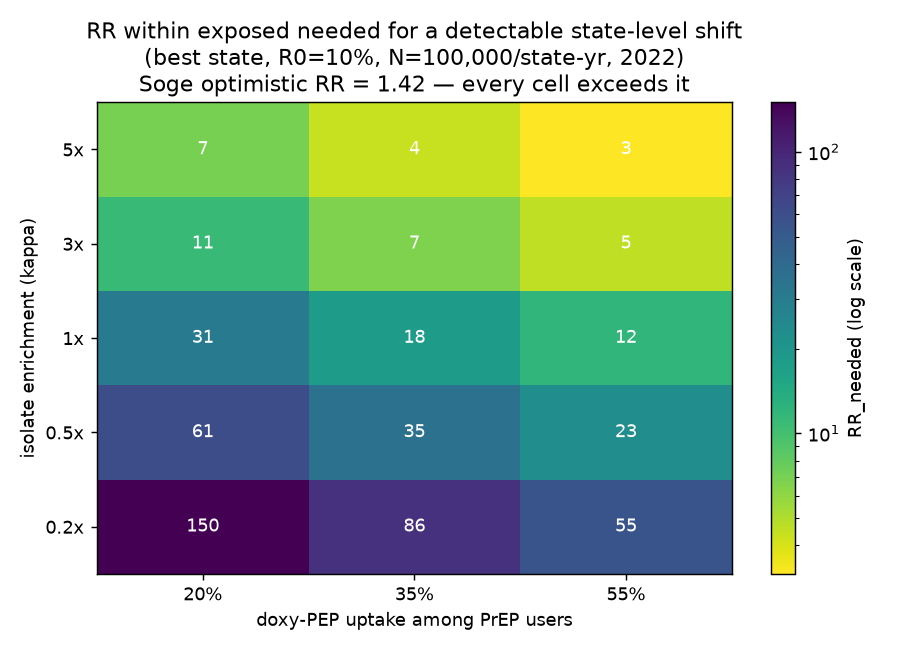
\includegraphics[keepaspectratio,alt={Figure 1. State level. Within-exposed relative risk required for a detectable state-level shift in tetracycline non-susceptibility, over doxy-PEP uptake × isolate enrichment (best state, R₀ = 10\%, N = 100 000/state-year). Every cell exceeds Soge's optimistic RR = 1.42.}]{../outputs/figures/feasibility_dilution.png}}
\caption{\textbf{Figure 1.} State level. Within-exposed relative risk
required for a detectable state-level shift in tetracycline
non-susceptibility, over doxy-PEP uptake × isolate enrichment (best
state, R₀ = 10\%, N = 100 000/state-year). Every cell exceeds Soge's
optimistic RR = 1.42.}
\end{figure}

\begin{figure}
\centering
\pandocbounded{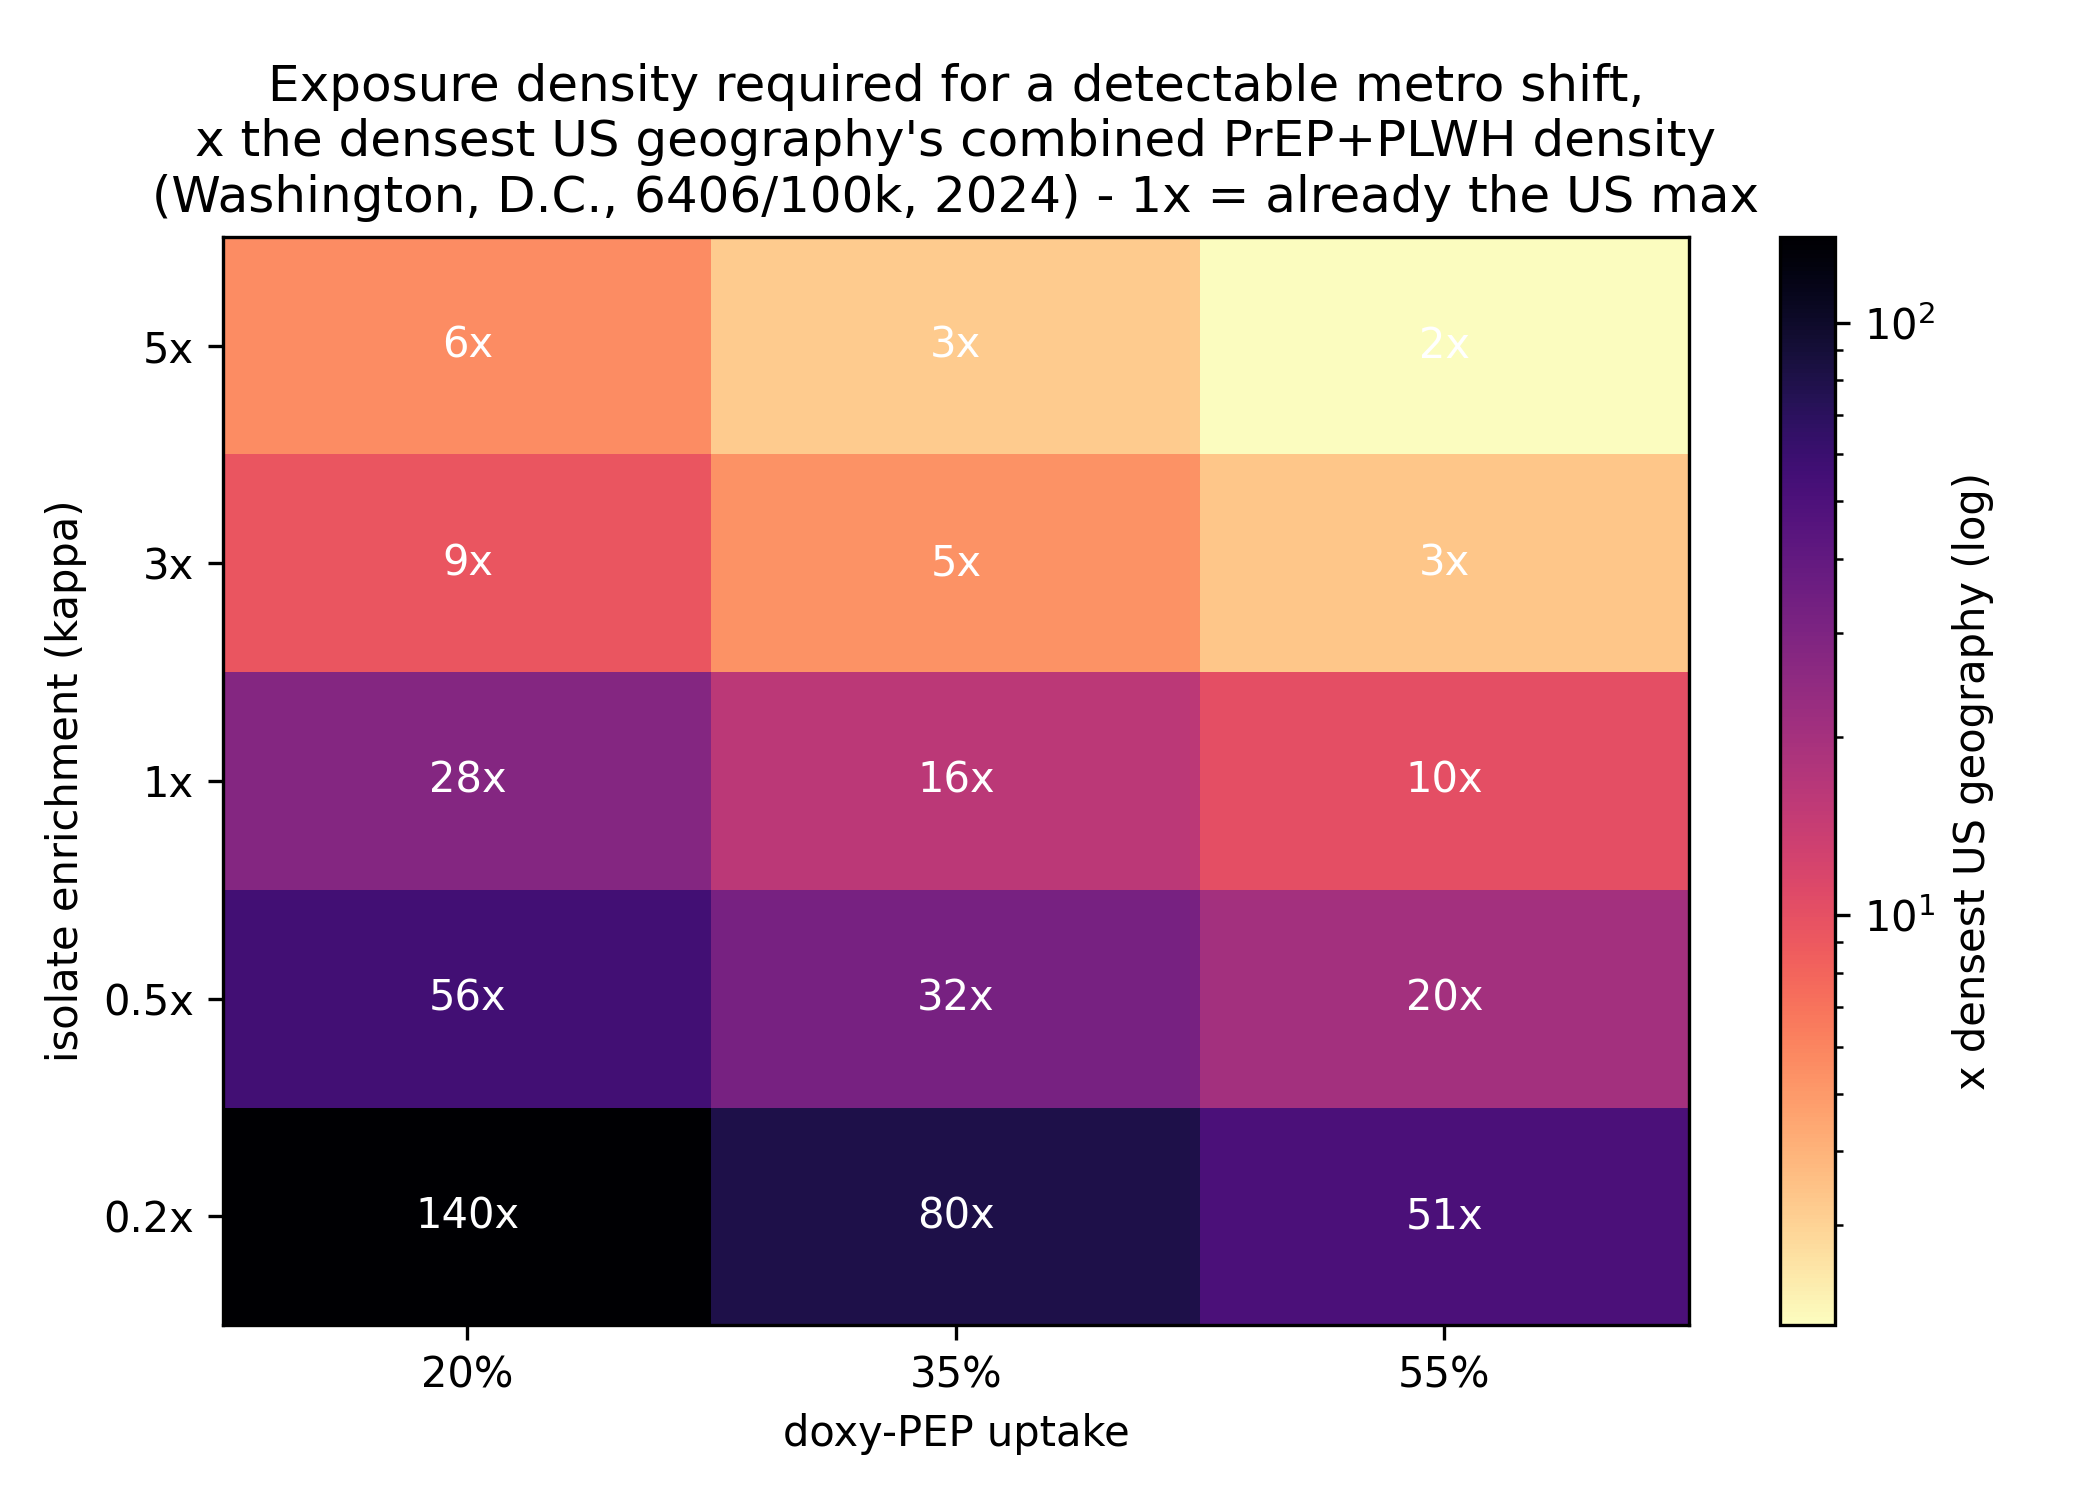
\includegraphics[keepaspectratio,alt={Figure 2. Metro level. Male-PrEP density required for a detectable shift, as multiples of the densest US geography (Washington, D.C.). 1× is already the national maximum.}]{../outputs/figures/feasibility_metro.png}}
\caption{\textbf{Figure 2.} Metro level. Male-PrEP density required for
a detectable shift, as multiples of the densest US geography
(Washington, D.C.). 1× is already the national maximum.}
\end{figure}

\begin{figure}
\centering
\pandocbounded{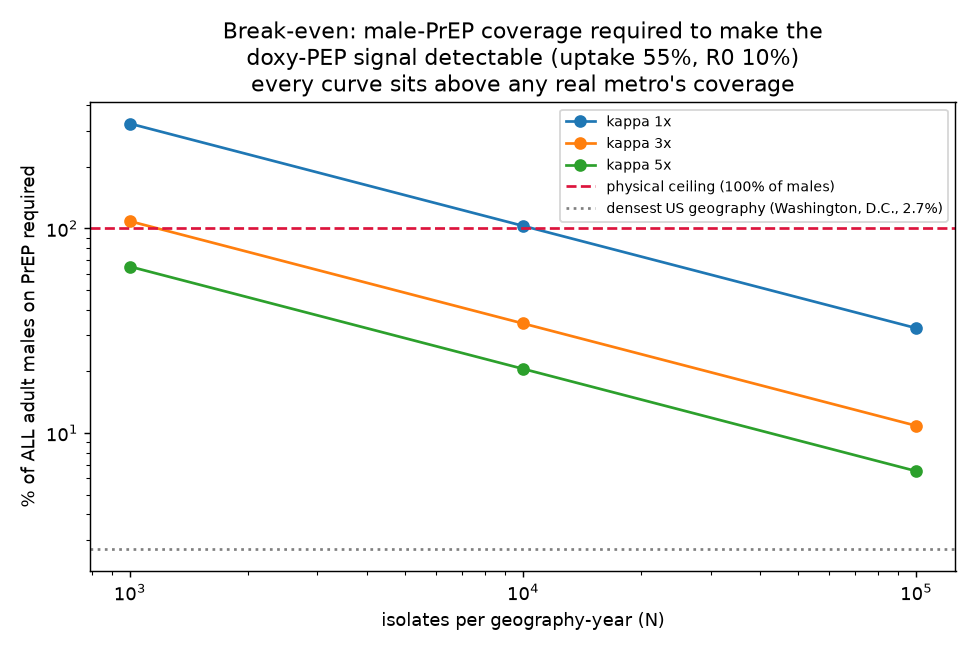
\includegraphics[keepaspectratio,alt={Figure 3. Break-even in proxy-free units. Share of all adult males on PrEP required for detection versus isolates per geography-year, by enrichment κ. Every curve sits above D.C.'s observed 2.7\% and, under realistic isolate volumes, above the 100\%-of-males physical ceiling.}]{../outputs/figures/feasibility_metro_breakeven.png}}
\caption{\textbf{Figure 3.} Break-even in proxy-free units. Share of
\emph{all} adult males on PrEP required for detection versus isolates
per geography-year, by enrichment κ. Every curve sits above D.C.'s
observed 2.7\% and, under realistic isolate volumes, above the
100\%-of-males physical ceiling.}
\end{figure}

\subsection{Declarations}\label{declarations}

\textbf{Data and code availability.} All data are public (AIDSVu;
published trials, guidelines, and the CROI abstract) and all analysis
code is in the project repository, which regenerates every figure and
table via \texttt{make\ all}. Every coded source is SHA-256--pinned. No
restricted-access data were used.

\textbf{Conflicts of interest.} A.C.D. reports former employment at
Gilead Sciences (01/2020--11/2024) with prior ownership of corporate
stock, all divested by 12/2024; Gilead played no role in this work.
A.C.D. is sole owner of Nyx Dynamics LLC. This work was completed
independently of any funding.

\textbf{Use of artificial intelligence.} A large language model was used
for writing and analysis-engineering assistance beyond copyediting. The
scientific argument, the close reading of the primary sources, the model
specification, and all conclusions are the author's own; the author
reviewed all generated content, independently verified every numerical
value and quotation against primary sources and the regenerable analysis
outputs, and takes full responsibility. No AI tool is credited as an
author.

\textbf{Funding.} None.

\subsection*{References}\label{references}
\addcontentsline{toc}{subsection}{References}

\protect\phantomsection\label{refs}
\begin{CSLReferences}{1}{1}
\bibitem[\citeproctext]{ref-aidsvu}
AIDSVu. 2026. \emph{State and County {PrEP} Use and {PrEP}-to-Need
Ratio, 2012--2025}. Emory University, Rollins School of Public Health.
\url{https://aidsvu.org}.

\bibitem[\citeproctext]{ref-cdc2024doxypep}
Centers for Disease Control and Prevention. 2024. \emph{Guidelines for
the Use of Doxycycline Postexposure Prophylaxis for Bacterial Sexually
Transmitted Infection Prevention}. MMWR Recomm Rep.

\bibitem[\citeproctext]{ref-demidont2026metaarxiv}
{Demidont, Adrian C., and {[}coauthor{]} Farina}. 2026. \emph{A
150-Journal Audit of Computational-Reproducibility Policy: Fifty Policy
Units, Zero Code or Runnable-Artifact Mandates}. MetaArXiv preprint.

\bibitem[\citeproctext]{ref-diep2008}
Diep, Binh An, Henry F. Chambers, Christopher J. Graber, et al. 2008.
{``Emergence of Multidrug-Resistant, Community-Associated,
Methicillin-Resistant {Staphylococcus aureus} Clone {USA300} in Men Who
Have Sex with Men.''} \emph{Ann Intern Med} 148 (4): 249--57.

\bibitem[\citeproctext]{ref-grossman2016}
Grossman, Trudy H. 2016. {``Tetracycline Antibiotics and Resistance.''}
\emph{Cold Spring Harb Perspect Med} 6 (4): a025387.

\bibitem[\citeproctext]{ref-dejong2025}
{Jong, N. de et al.} 2025. {``Community-Acquired Methicillin-Resistant
{Staphylococcus aureus} ({CA-MRSA}) in Men Having Sex with Men ({MSM}):
A Systematic Review of Risk Factors, Prevalence, and Transmission.''}
\emph{BMC Infect Dis} 25: 299.

\bibitem[\citeproctext]{ref-liu2011}
Liu, Catherine, Arnold Bayer, Sara E. Cosgrove, et al. 2011. {``Clinical
Practice Guidelines by the {Infectious Diseases Society of America} for
the Treatment of Methicillin-Resistant {Staphylococcus aureus}
Infections in Adults and Children.''} \emph{Clin Infect Dis} 52 (3):
e18--55.

\bibitem[\citeproctext]{ref-luetkemeyer2023}
{Luetkemeyer, Anne F., Deborah Donnell, Julia C. Dombrowski, et al.}
2023. {``Postexposure Doxycycline to Prevent Bacterial Sexually
Transmitted Infections.''} \emph{N Engl J Med} 388: 1296--306.

\bibitem[\citeproctext]{ref-luetkemeyer2023croi}
Luetkemeyer, Anne F., and DoxyPEP Study Team. 2023. \emph{{DoxyPEP} and
Antimicrobial Resistance in {N. gonorrhoeae}, Commensal {Neisseria} and
{S. aureus}}. Conference on Retroviruses and Opportunistic Infections
(CROI), Oral Abstract OA-3.

\bibitem[\citeproctext]{ref-miko2012}
{Miko, Benjamin A. et al.} 2012. {``High Prevalence of Colonization with
{Staphylococcus aureus} Clone {USA300} at Multiple Body Sites Among
Sexually Transmitted Disease Clinic Patients: An Unrecognized
Reservoir.''} \emph{Microbes Infect} 14 (12): 1040--43.

\bibitem[\citeproctext]{ref-sfdph2022}
San Francisco Department of Public Health. 2022. \emph{Health Update:
Doxycycline Post-Exposure Prophylaxis (Doxy-PEP) for Prevention of
Bacterial {STIs}}.

\bibitem[\citeproctext]{ref-soge2025}
{Soge, Olusegun O., Christina S. Thibault, Chase A. Cannon, et al.}
2025. {``Potential Impact of Doxycycline Post-Exposure Prophylaxis on
Tetracycline Resistance in {Neisseria gonorrhoeae} and Colonization with
Tetracycline-Resistant {Staphylococcus aureus} and {Group A
Streptococcus}.''} \emph{Clin Infect Dis} 80: 1188--96.

\bibitem[\citeproctext]{ref-stevens2014}
Stevens, Dennis L., Alan L. Bisno, Henry F. Chambers, et al. 2014.
{``Practice Guidelines for the Diagnosis and Management of Skin and Soft
Tissue Infections: 2014 Update by the {Infectious Diseases Society of
America}.''} \emph{Clin Infect Dis} 59 (2): e10--52.

\end{CSLReferences}

\end{document}
